\documentclass{beamer}
\usepackage[ngerman]{babel}
\usepackage{amsmath}
\usepackage{url}
\usepackage{graphicx}
\usepackage{scalerel}
\usepackage{nameref}
\usepackage{siunitx}
\usepackage[justification=raggedright, font=scriptsize, skip=2pt, belowskip=0pt]{caption}
\usepackage[bottom]{footmisc}
\usepackage[backend=biber, style=verbose]{biblatex}
\usepackage{csquotes}
\usepackage{animate}


\addbibresource{bibliography.bib}

\renewcommand{\thefootnote}{\arabic{footnote}}
\renewcommand{\thempfootnote}{\arabic{mpfootnote}}
% \footnote[frame] glues the footnote to the bottom of the frame even in minipage/column environments
\newcommand{\myfootcite}[1]{\footnote[frame]{\cite{#1}}}
% make footnotes smaller size else to much text in each frame
\let\oldfootnotesize\footnotesize
\renewcommand*{\footnotesize}{\oldfootnotesize\scriptsize}


\usetheme[width=1.9cm]{Hannover}
\usecolortheme{seagull}

%opening
\title{Filterung von Frequenzen in \\WAV-Audio Dateien \\ mithilfe der Fourier Transformation}
\author{Len-Marvin Adler}
\institute{Hochschule Bonn-Rhein-Sieg}
\date{\today}
%\titlegraphic{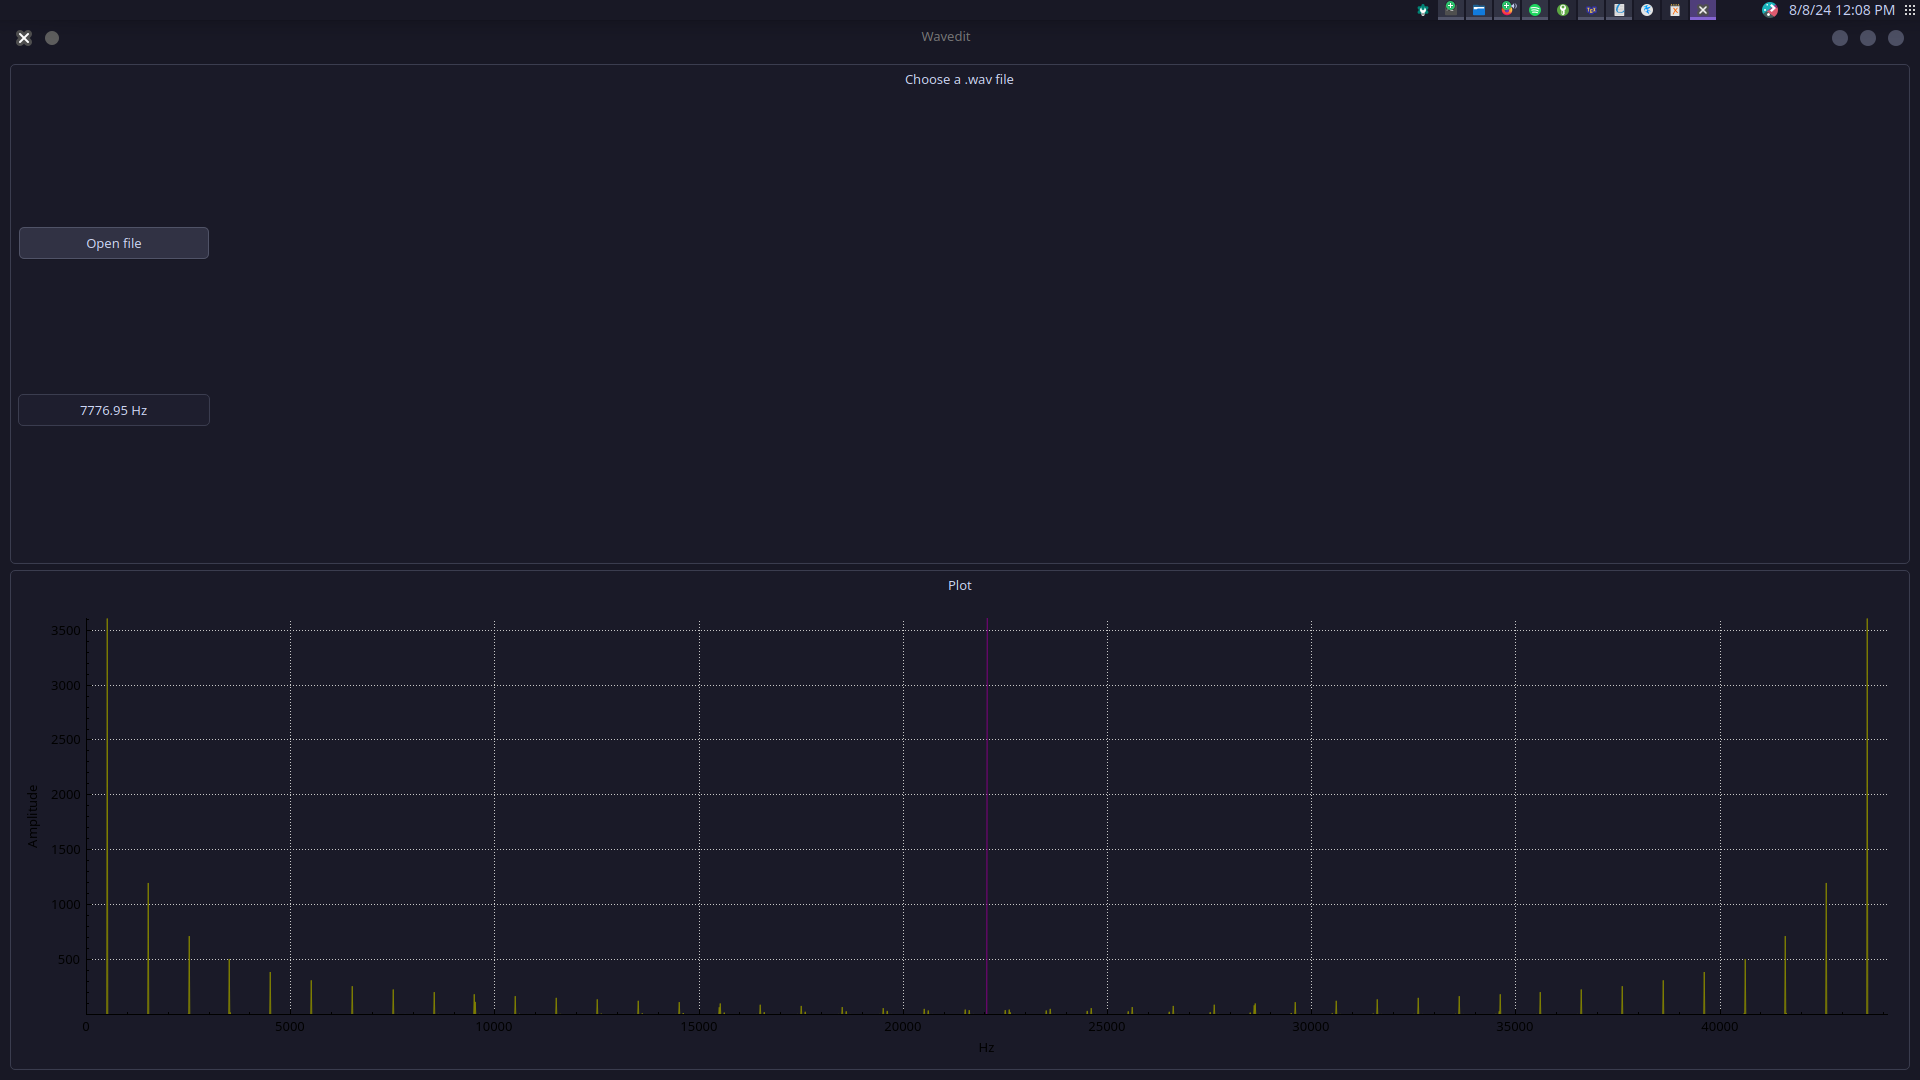
\includegraphics[height=0.3\textheight]{images/sqr500Hz.png}}

\setbeamercolor{itemize item}{fg=lightgray}
\setbeamertemplate{itemize item}[triangle]

\setbeamertemplate{section in toc}[square]
\setbeamertemplate{subsection in toc}{\hspace{2em}{\color{lightgray}\rule[0.3ex]{3pt}{3pt}}~\inserttocsubsection\par}

\def\smarginleft{1.9cm}
\setbeamertemplate{sidebar left}
{
  {\usebeamerfont{title in sidebar}
    \vskip1.5em
    \usebeamercolor[fg]{title in sidebar}
    \insertshorttitle[width=\smarginleft,center,respectlinebreaks]\par
    \vskip1.25em
  }
  \hbox to2cm{\hss\insertlogo\hss}
  \vskip1.25em
  \insertverticalnavigation{\smarginleft}
  \vfill
  \hbox to2cm{\hskip0.8cm\usebeamerfont{subsection in
      sidebar}\strut\usebeamercolor[fg]{subsection in
      sidebar}\insertframenumber-\inserttotalframenumber\hfill}
  \vskip3pt
}

\begin{document}

\frame{\titlepage}

\section*{Inhaltsverzeichnis}
\begin{frame}{Inhaltsverzeichnis}
	\tableofcontents
\end{frame}

%% 1.
\section{Begriffe der Digitalen Signalverarbeitung}
\begin{frame}{Begriffe der Digitalen Signalverarbeitung}
	%Nur wichtigste Punkte als Auflistung
	\begin{itemize}
		\vspace{0.75em}
		\item Signale sind immer diskret \vspace{0.5em}
		\item Nyquist-Shannon-Abtasttheorem\myfootcite{dspguide:3:nyquist}: $f_{abtast} > 2 \cdot \hat{f}_{signal}$ 
		\\ sonst tritt Alias-Effekt auf \vspace{0.5em}
		\begin{figure}
			\raggedright
			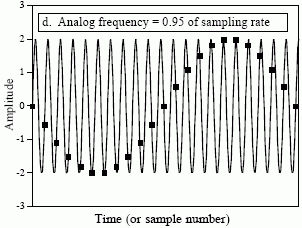
\includegraphics[width=0.35\textwidth]{images/alias-effekt2.png}
		\end{figure}
		\item Nyquist-Frequenz $f_{Nyquist} := \frac{1}{2} f_{abtast}$
		\\ $\Rightarrow$ also $\hat{f}_{signal} < f_{Nyquist}$  \vspace{0.5em}
		% Abtastrate muss größer sein als 2 * die höchste Frequenz die im Signal vorkommt,
		% damit das Signal korrekt rekonstruiert werden kann,
		% sonst kommt es zum Alias-Effekt
	\end{itemize}
\end{frame}

 


%% 2.
\section{WAV Datei}
\begin{frame}{\insertsection}
	%Nur wichtigste Punkte als Auflistung
	\begin{columns}[T]
		\begin{column}{0.6\textwidth}
			\vspace{1em}
			\begin{itemize}
				\item basiert auf RIFF Dateiformat von Microsoft
				\item besteht aus den $3$ Subchunks\myfootcite{WAV-Header}
				\begin{itemize}
					\item 'RIFF': enthält die Information, dass es sich um eine RIFF WAVE Datei handelt \vspace{0.25em}
					\item 'fmt ': enthält Informationen über die Daten, wie z.B SampleRate, BitsPerSample \vspace{0.25em}
					% Qualität der Audio wird durch SampleRate, BitsPerSample bestimmt
					\item 'data': enthält Datenwerte
				\end{itemize}
			\end{itemize}
		\end{column}
		\hfill
		\begin{column}{0.4\textwidth}
			\begin{figure}
				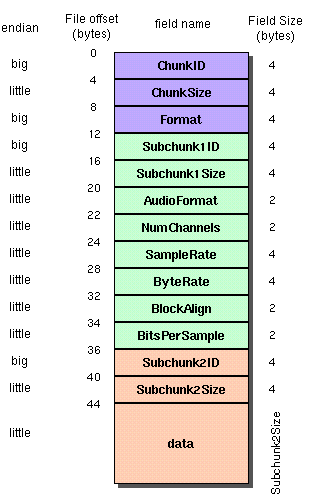
\includegraphics[scale=0.4]{images/wav-header.png}
				\caption{\centering \scriptsize WAV-Header\footnotemark[\thefootnote]}
			\end{figure}
		\end{column}
	\end{columns}
\end{frame}


\begin{frame}{\insertsection}
	\begin{figure}
		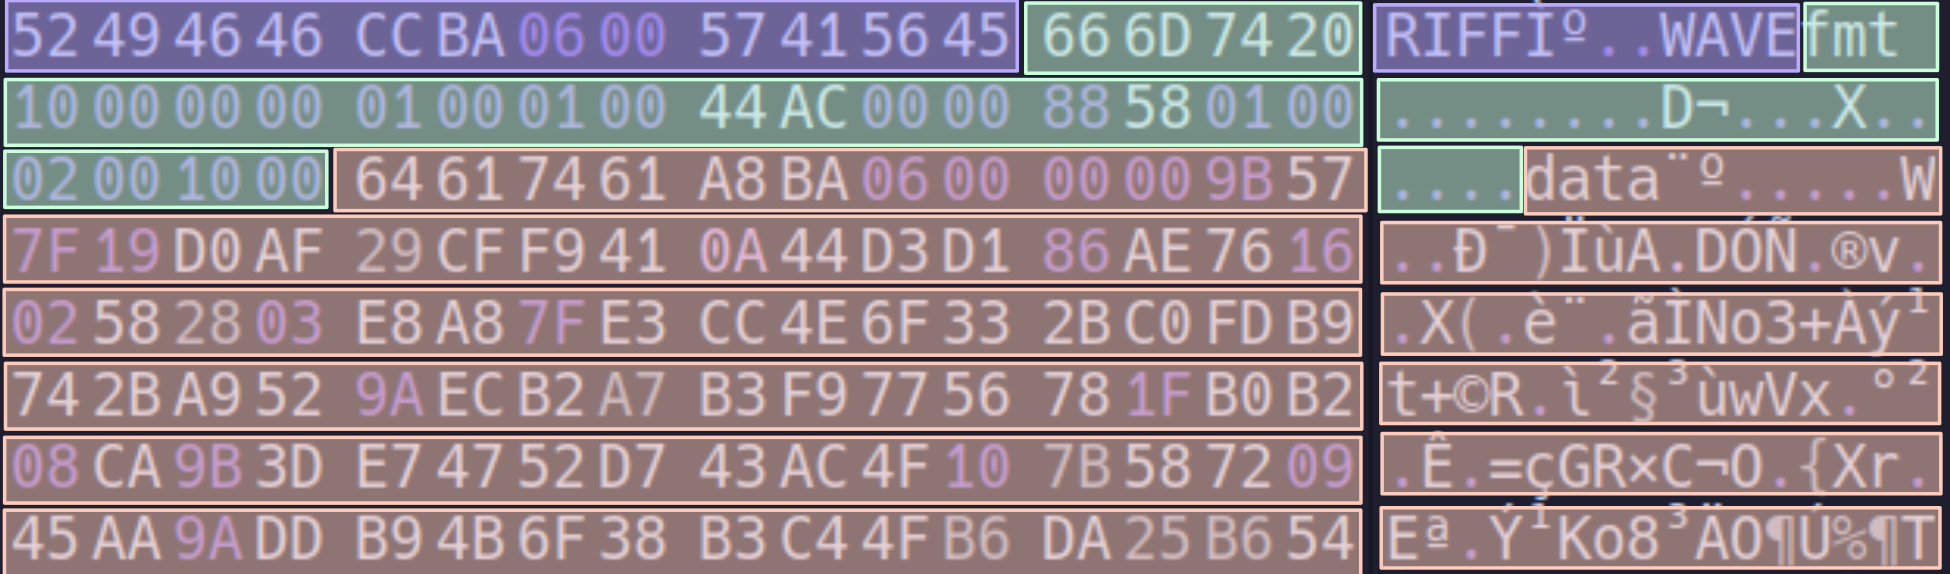
\includegraphics[scale=0.15]{images/wav_hex.png}
		\caption{\centering Ausschnitt einer WAV Datei mit markierten Subchunks,\\dargestellt in einem Hex-Editor}
	\end{figure}
	\begin{itemize}
		\item Abtastrate ist oft $\SI{44.1}{\kilo\hertz}$ \myfootcite{44100Hz},
		\\  Menschen hören Töne im Bereich $\SI{20}{\hertz}-\SI{20}{\kilo\hertz}$ \myfootcite{MenschlicheHoerfrequenz}
		\item Analoges Signal wird durch lineare Pulse Code Modulation (PCM)  in ein digitales Signal umgewandelt (verlustfrei)
	\end{itemize}
\end{frame}

%% 3.
\section{Fourier Transformation}
\subsection{DFT, FFT}
\begin{frame}{\insertsection}
	\framesubtitle{\insertsubsection}
	\begin{itemize}
		\item DFT: Fourier-Koeffizienten $\beta_j = \sum\limits_{k=0}^{n-1} x_k e^{-2\pi i \frac{jk}{n}} \enspace ; j=0,\ldots,n-1$ \blfootnote{stoerBulirsch}
		\item FFT: Voraussetzung $n = 2^\psi; \psi \in \mathbb{N}_0$ (Radix-2-FFT)
		% Wenn Voraussetzung mit gegebenen Daten nicht erreicht, hänge soviele 0 an die Daten hinten ran
		% bis die Anzahl eine Zweierpotenz ist, 0 fügen keinen Frequenzanteil bzw. keine Informationen hinzu
		\\ $\Rightarrow$ Divide-and-Conquer, berechne Fourier-Koeffizienten \\ \hskip 1.35em in $2$ Hälften \\
		Sei $m = \frac{n}{2}; \enspace \varepsilon_\psi = e^{-\frac{2\pi i}{2^\psi}}$ \newline
		\small{$\beta_{2\kappa} = \sum\limits_{k=0}^{m-1} (x_k+x_{k+m})\varepsilon_{\psi-1}^{\kappa k} ; \enspace \kappa = 0,\ldots,m-1$}
		\small{$\beta_{2\kappa+1} = \sum\limits_{k=0}^{m-1} ((x_k-x_{k+m})\varepsilon_{\psi}^{\kappa k})\varepsilon_{\psi-1}^{\kappa k}$}
		%\\ $\Rightarrow$ u.a. $\varepsilon_{\psi-1}^{\kappa k}$ kommt in beiden Gleichungen vor \vspace{0.5em}
		\vspace{0.5em}
		\\ $\Rightarrow$ insgesamt halbiert sich der Rechenaufwand pro $\beta_j$
	\end{itemize}
\end{frame}

\begin{frame}{\insertsection}
	\framesubtitle{\insertsubsection}
	\begin{itemize}
		\item DFT ist konjugiert symmetrisch\myfootcite{conjugateSymmetry}, \\ wenn Datenwerte $x_j \in \mathbb{R}$ %sind
		\begin{align*}
			\beta_{n-j} & = \sum\limits_{k=0}^{n-1} x_k \cdot e^{-2\pi i \frac{(N-j)k}{n}} =  \sum\limits_{k=0}^{n-1} x_k \cdot \overline{e^{-2\pi i \frac{jk}{n}}} \\
			& =  \overline{\sum\limits_{k=0}^{n-1} x_k \cdot e^{-2\pi i \frac{jk}{n}}} = \overline{\beta_j}
			% funktioniert nur wenn x_j reell damit Im(x_j) = 0 ist und somit x_j = Conj(x_j)
		\end{align*}
		\\ $\Rightarrow$ es reicht DFT von Datenwerten $x_j$ \\ \hskip 1.35em mit $j \in [0,n/2]$ zu berechnen
	\end{itemize}
\end{frame}

\subsection{Performance}
\begin{frame}{\insertsection}
	\framesubtitle{\insertsubsection}

	\begin{columns}[T] % align columns{\tiny }
	\begin{column}{0.6\textwidth}
		\begin{figure}
			\centering
			\includegraphics[scale=0.3]{images/Runtime\_DFT\_FFT\_1e6.png}
			%\caption{\centering Laufzeitverhalten von \\ DFT, FFT}
		\end{figure}
		\begin{itemize}
			\item Jede Iteration berechnet $e^{-2\pi i \frac{jk}{n}}$
			\\ $\rightarrow$ Benchmark\myfootcite{Benchmark-std::exp}: ca. $\SI{5}{\nano\second}$
		\end{itemize}
	\end{column}
	\hfill
	\begin{column}{0.48\textwidth}
		\begin{itemize}
			\vspace{1em}
			\item[] Für $n=10^6$, also eine WAV Datei mit $10^6$ Datenwerten ($\SI{2}{\mega\byte}$) gilt:
			\item DFT $ \approx 10^{12}$ Iterationen
			\\ $\Rightarrow$ Berechnung dauert ca. $10^{12} \cdot \SI{5}{\nano\second} = \SI{5000}{\second} \newline \approx \SI{83}{\minute}$ 
			\item FFT $ \approx 10^{7}$ Iterationen
			\\ $\Rightarrow$ Berechnung dauert ca. $10^{7} \cdot \SI{5}{\nano\second} = \SI{0.05}{\second}$
		\end{itemize}
	\end{column}
	\end{columns}
\end{frame}


\subsection{Frequency bins}
\begin{frame}{\insertsection}
	\framesubtitle{\insertsubsection}
	\begin{itemize}
		\item Frequenzen werden in bins zusammengefasst durch \blfootnote{frequencyBins}
					$f_i = i \cdot \frac{f_{abtast}}{n}$
		\item[] z.B. für $f_{abtast} = \SI{44.1}{\kilo\hertz}, n=1024$ \\ \vspace{0.25em}
		$\begin{matrix}
			0: & 0 \cdot \SI{44100}{\hertz} / 1024 & = &  \SI{0.0}{\hertz}  \\
			1: & 1 \cdot \SI{44100}{\hertz} / 1024 & = &  \SI{43.1}{\hertz} \\
			2: & 2 \cdot \SI{44100}{\hertz} / 1024 & = &  \SI{86.1}{\hertz} \\
			& \ldots \\
			512: & 512 \cdot \SI{44100}{\hertz} / 1024 & = & \SI{22050}{\hertz} \\
			& \ldots
		\end{matrix}$ \vspace{0.5em}
		\\ $\Rightarrow$ Je mehr Datenpunkte, desto schmaler \\ \hskip 1.35em werden die frequency bins
		\item Nyquist-Frequenz gehört zu Bin $n/2$
		\item Frequenzspektrum: Frequenz $f_i$ hat Amplitude $|\beta_i|$
	\end{itemize}
\end{frame}

\subsection{IDFT}
\begin{frame}{\insertsection}
	\framesubtitle{\insertsubsection}
	
	\begin{itemize}
		\item im Grunde ist IDFT nur eine DFT mit Normalisierungsfaktor
		\\ $x_j = \frac{1}{n} \sum\limits_{k=0}^{n-1} \beta_k e^{2\pi i \frac{jk}{n}} \enspace ; j=0,\ldots,n-1$ \vspace{0.5em}
		\item Matrix-Schreibweise: \\ %\vspace{0.25em}
		$\begin{bmatrix}
			\omega^{jk}
		\end{bmatrix}
		\begin{bmatrix}
			\omega^{jk}
		\end{bmatrix}^\dag
		= n \cdot E_n
		\enspace; j,k=0,\ldots,n-1$
		\item[] mit $\omega = e^{-2\pi i \frac{1}{n}}$
		%\vspace{0.5em}
		\item auch IFFT existiert um IDFT zu berechnen
	\end{itemize}
\end{frame}


\subsection{Konvergenzverhalten, Fehleranalyse}
\begin{frame}{\insertsection}
	\framesubtitle{\insertsubsection}
	\begin{itemize}
		\vspace{1em}
		\item Fourier-Reihe konvergiert punktweise\myfootcite{KonvergenzFourierReihe},
		\\ gleichmäßige Konvergenz in kompakten Intervallen in denen $f(t)$ stetig ist
		\item Gibbssches Phänomen: Überschwingung an Unstetigkeitsstellen um mind. $9\%$ bei abgebrochener Fourier-Reihe
	\end{itemize}
	\begin{figure}
		\centering
		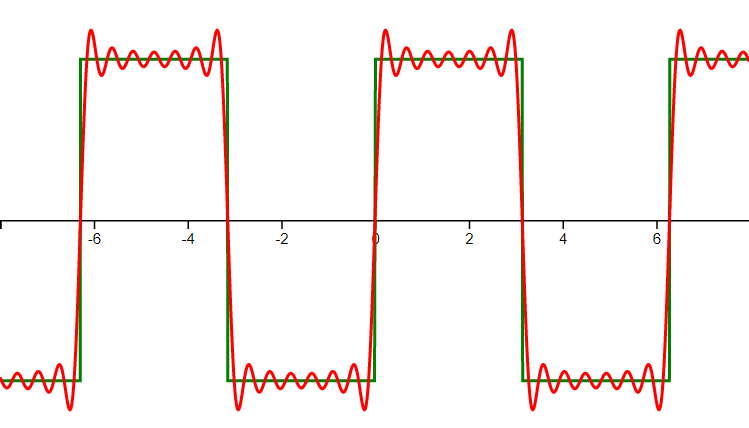
\includegraphics[scale=0.15]{images/gibbs.png}
		\caption*{\centering Gibbsches Phänomen, \\ \href{https://resources.altium.com/de/p/how-gibbs-phenomenon-produces-measurement-artifacts}{https://resources.altium.com/de/p/how-gibbs-phenomenon-produces-measurement-artifacts}}
	\end{figure}
\end{frame}

\begin{frame}{\insertsection}
	\framesubtitle{\insertsubsection}
	\begin{itemize}
		\item DFT als Matrix ist eine Vandermonde-Matrix: \\ \vspace{0.5em}
		$\begin{bmatrix}
			1 & 1 & 1 & \cdots & 1 \\
			1 & \omega & \omega^2 & \cdots & \omega^{n-1} \\
			1 & \omega^2 & (\omega^2)^2 & \cdots & (\omega^2)^{n-1} \\
			\vdots & \vdots & \vdots & \ddots & \vdots \\
			1 & \omega^{n-1} & (\omega^{n-1})^2 & \cdots & (\omega^{n-1})^{n-1} \\
		\end{bmatrix} $ \vspace{0.5em}
		\item Vandermonde-Matrizen sind grundsätzlich schlecht konditioniert,
		%$det = \prod\limits_{0 \le i < j \le n} (x_j - x_i)$
		Ausname: DFT ist gut konditioniert\myfootcite{VandermondeCondition}
	\end{itemize}
\end{frame}


\subsection{Leck-Effekt, Fensterfunktionen}
\begin{frame}{\insertsection}
	\framesubtitle{\insertsubsection}
	
	\begin{itemize}
		\item Anzahl der Datenpunkte eines zeitdiskreten Signals ist kein ganzzahliges Vielfaches der Periodendauer
		% sehr wahrscheinlich dass der Fall eintritt
		\item DFT gibt Frequenzanteile an, die im unendlich langen Signal nicht vorkämen
		\item Leck-Effekt (spectral leakage) tritt auf, weil das Signal nur endlich lange beobachtet werden kann
	\end{itemize}
	
	\begin{columns}[T] % align columns{\tiny }
		\begin{column}{0.48\textwidth}
			\begin{figure}
				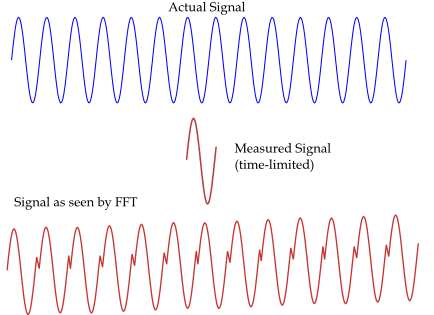
\includegraphics[scale=0.25]{images/spectralLeakage.png}
				\caption*{\centering Zustandekommen des Leck-Effekts, \href{https://www.gaussianwaves.com/2011/01/fft-and-spectral-leakage-2/}{\tiny https://www.gaussianwaves.com/2011/01/fft-and-spectral-leakage-2/}}
			\end{figure}
		\end{column}
		\hfill
		\begin{column}{0.5\textwidth}
			\begin{figure}
				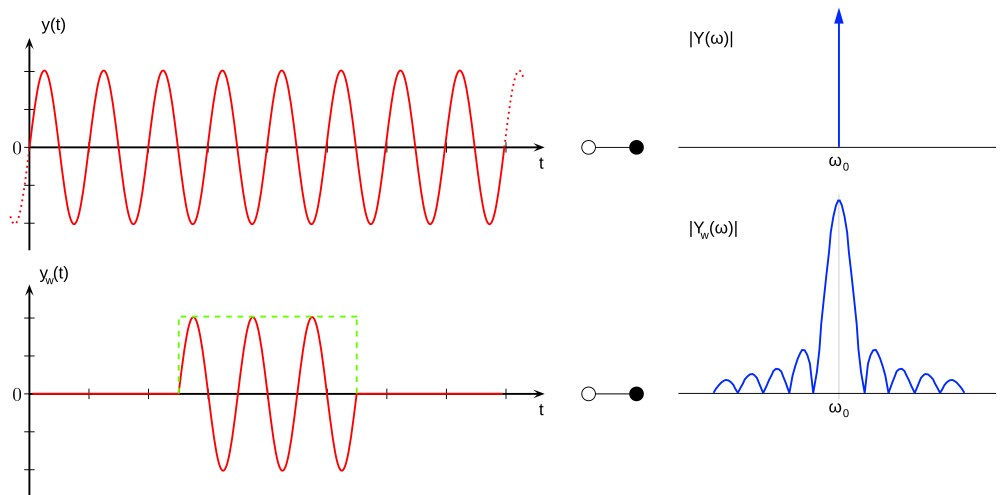
\includegraphics[scale=0.185]{images/spectralLeakage-WindowFunction.png}
				\caption*{\centering implizite Anwendung eines Rechteck-Fensters, \href{https://de.wikipedia.org/wiki/Leck-Effekt}{\tiny https://de.wikipedia.org/wiki/Leck-Effekt}}
			\end{figure}
		\end{column}
	\end{columns}
\end{frame}

\begin{frame}{\insertsection}
	\framesubtitle{\insertsubsection}
	
	\begin{itemize}
		\vspace{1em}
		\item Leck-Effekt lässt sich nicht komplett vermeiden
		\item Auswirkung aber reduzierbar durch Fensterfunktionen
		\item Fensterfunktion wird vor der DFT Operation auf das Signal angewendet, sodass das Signal
				  künstlich periodisiert wird
				  % wenn man kein Fenster verwendet wird implizit das Rechteck-Fenster (Daten*1) angewendet,
				  % weil die Daten nur endlich lang sind
				  % Faltungssatz: Multiplikation im Zeitbereich ist Faltung der Fourier Transformierten und andersherum
				  % => Frequenzspektrum ist die Faltung aus DFT(Daten), DFT(Rechteck)
				  % wobei DFT(Rechteck) die Sinc-Funktion ist und diese hat Ripples
	\end{itemize}
	\begin{figure}
		\centering
		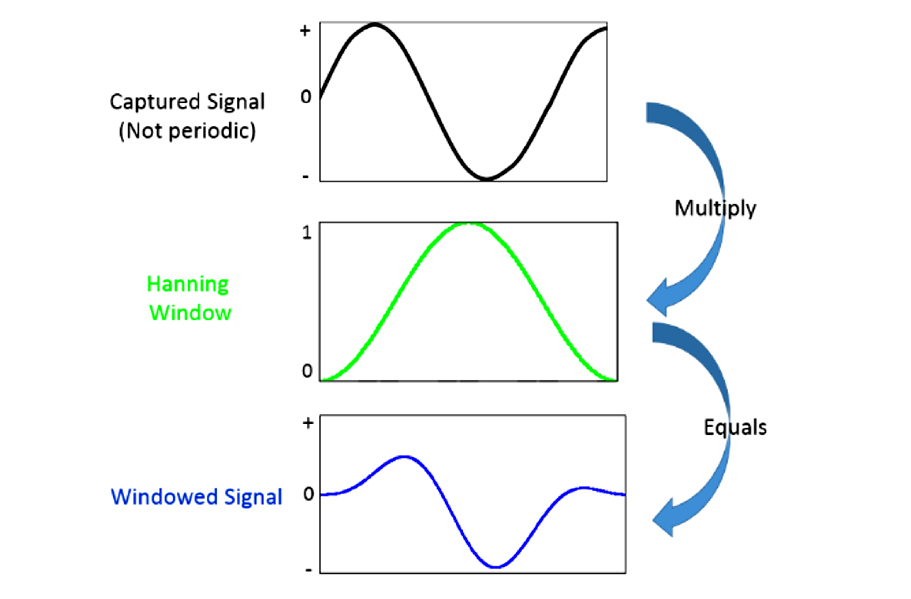
\includegraphics[scale=0.4]{images/appliedWindowFunction2.jpg}
		\caption*{\centering Anwendung des Von-Hann-Fensters,\\ \href{https://www.modalshop.com/rental/learn/basics/how-to-choose-fft-window}{\tiny https://www.modalshop.com/rental/learn/basics/how-to-choose-fft-window}}
	\end{figure}
\end{frame}














 


%% 4.
\section{Frequenzen filtern}
\subsection{Vorgehensweise}
\begin{frame}{\insertsection}
	\framesubtitle{\insertsubsection}
	\begin{enumerate}
		\item Zeitdiskretes Signal durch DFT in Frequenzbereich überführen
		\item Amplitude der zu filternden Frequenzen auf $0$ setzen
		\item IDFT anwenden um das gefilterte zeitdiskrete Signal zu erhalten
	\end{enumerate}
\end{frame}

\subsection{Was kann schon schief gehen?}
\begin{frame}{\insertsection}
	\framesubtitle{\insertsubsection}
	\begin{itemize}
		\vspace{1em}
		\item Multiplizieren der zu filternden Frequenzanteile mit $0$ ist dasselbe wie Rechteck-Fenster anwenden
		\\ $\Rightarrow$ Faltungssatz greift erneut%\\ IDFT von Rechteck-Fenster ist wieder Sinc-Funktion
		\\ $\Rightarrow$ Frequenzanteile die nicht gefiltert werden sollen, \\ \hskip 1.35em werden auch (leicht) beeinflusst
	\end{itemize}
	\begin{figure}
		\includegraphics[height=0.3\textheight]{images/rectFilter\_impulseresponse.png}
		\caption*{\centering Idealer vs Realisierbarer Bandpass-Filter, \\ \href{https://dsp.stackexchange.com/a/37662}{https://dsp.stackexchange.com/a/37662}}
	\end{figure}
\end{frame}

\begin{frame}{\insertsection}
	\framesubtitle{\insertsubsection}
	\begin{itemize}
		\item Lösung: Fensterfunktion wird auf Rechteck-Fenster angewendet
		\item Frequenzen die nicht gefiltert werden sollen,\\ werden nun kaum beeinflusst
		\item filtert Frequenzen nicht auf $0$,\\ ein kleiner Frequenzanteil bleibt 
	\end{itemize}
\end{frame}

%% 5.
\section{Demonstration des Programms}
\begin{frame}{\insertsection}
	\begin{figure}
		\animategraphics[autoplay,loop,width=\linewidth]{30}{images/GIFs/cantina/cantina-}{1}{827}
		\caption*{Applikation \it{Wavedit}, Github: \href{https://github.com/gooosz/Wavedit.git}{https://github.com/gooosz/Wavedit.git}}
	\end{figure}
\end{frame}

% Nochmal als Bilder falls Gif zu schnell für Erklärungen war
\begin{frame}{\insertsection}
	\begin{figure}
		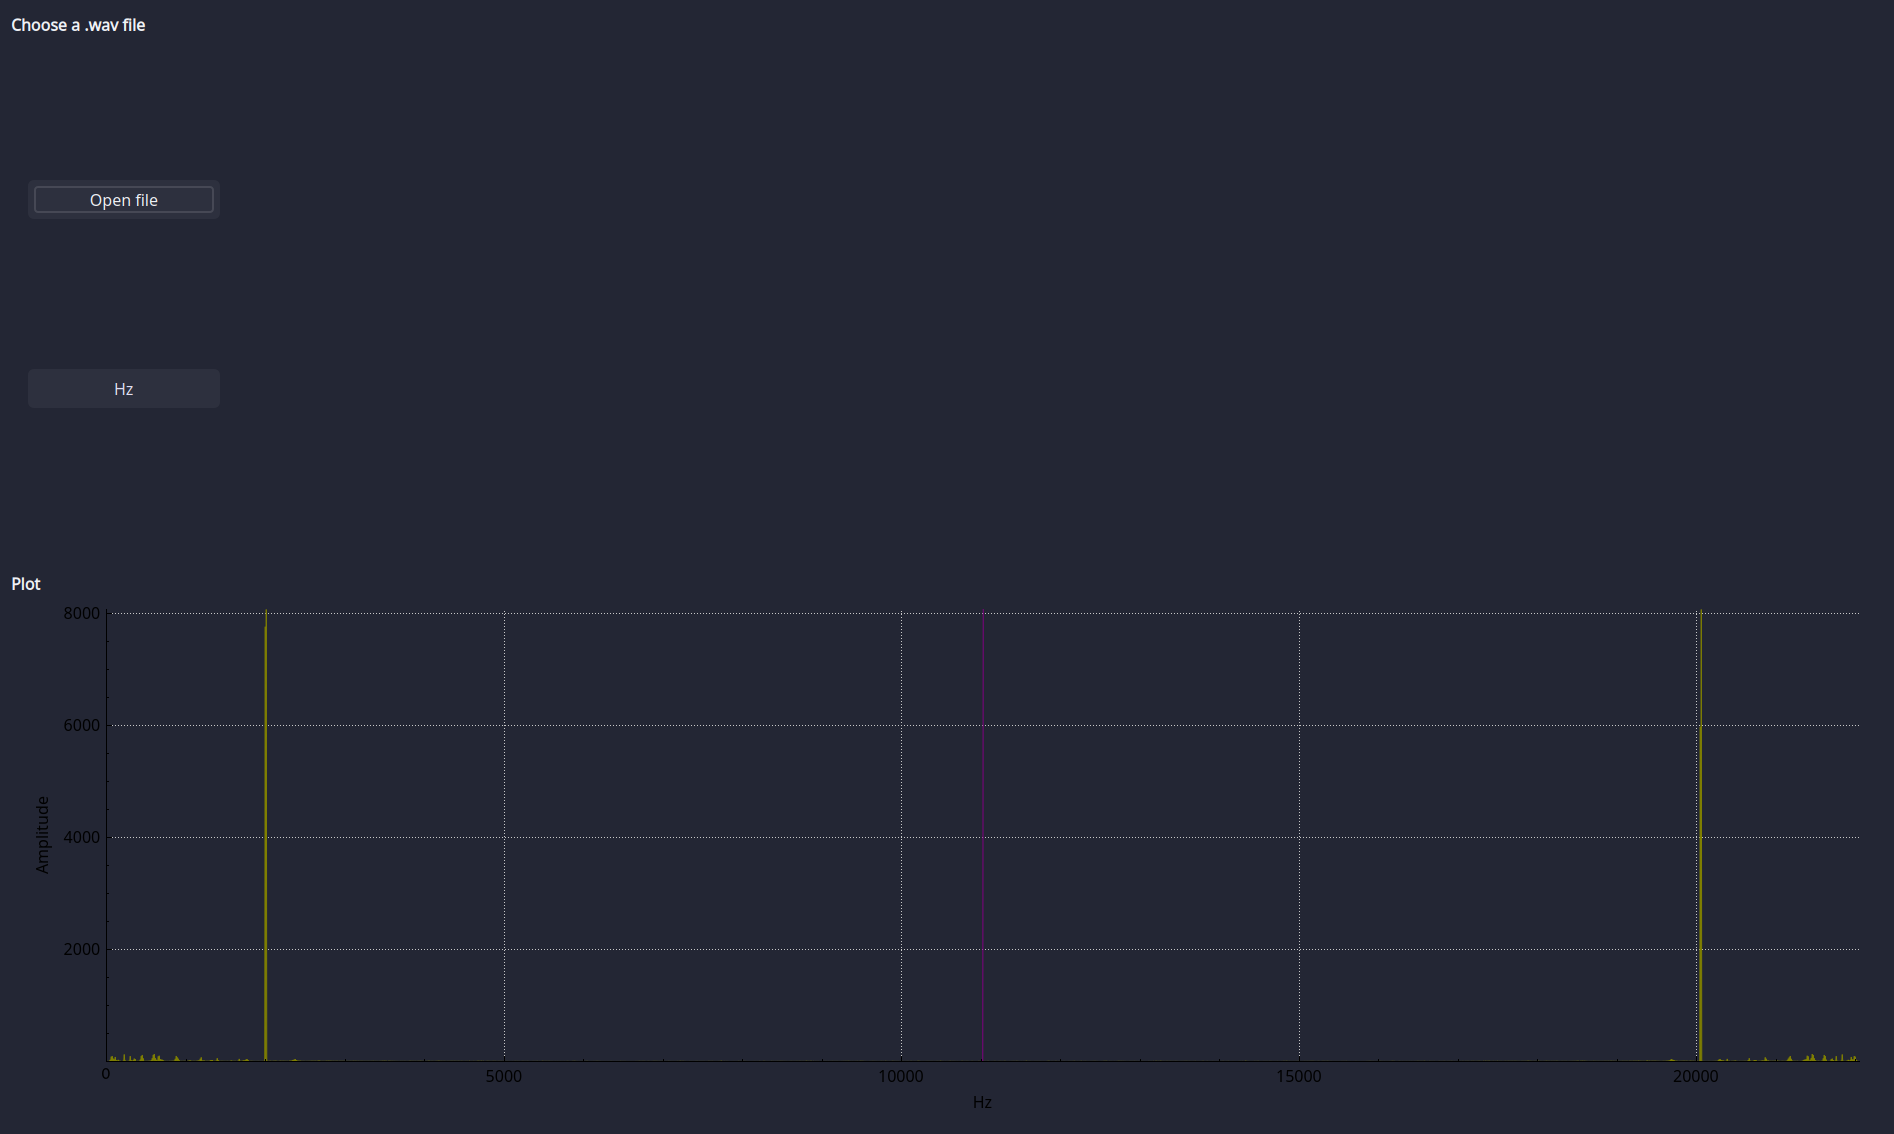
\includegraphics[width=\linewidth]{images/sin+cantina.png}
		\caption*{Frequenzspektrum von WAV Datei}
	\end{figure}
	% click on Play button to play the shown wav file
	\sound[]{Play audio}{audio/Sin440Hz_CantinaBand3.wav}
\end{frame}
\begin{frame}{\insertsection}
	\begin{figure}
		\includegraphics[width=\linewidth]{images/sin+cantina\_filtered.png}
		\caption*{Frequenzspektrum nach Filtern einer Frequenz von WAV Datei}
	\end{figure}
	% click on Play button to play the shown wav file
	\sound[]{Play audio}{audio/Sin440Hz_CantinaBand3.wav_filtered1995.63Hz.wav}
\end{frame}


%% 6.
\section{Fazit}
\begin{frame}{Fazit}
	\begin{itemize}
		\item Mithilfe der DFT lassen sich Frequenzen, die in der Tonspur einer WAV Datei auftreten, fast komplett herausfiltern
		\item Die Lautstärke der Audio wird dabei aber leicht gedämpft \vspace{0.5em}
		\\ $\Rightarrow$ Dennoch ist die Fourier Transformation ein \\ \hskip 1.35em effektives Werkzeug um Frequenzen zu filtern
	\end{itemize}

\end{frame}



%\printbibliography

\end{document}
